
\subsection{Model description}
The model is constructed as a rate network of two populations of neurons \textit{M} and \textit{V}, the former representing the memory trace of the \textit{K} available options (\textit{i.e.} the bandits), and the latter the value of the options under the current policy.
More formally, the model is defined by a set of coupled ordinary differential equations (ODEs).
The first equation tracks the evolution of the neural activity $\textbf{u}$ of population \textit{M}, while the second tracks the activity $\textbf{v}$ of the population \textit{V}. The time constant $\tau$ is the same for both equations and it is set to $10$ms.

\begin{equation}
\begin{aligned}
    \tau \dot{\textbf{u}}&= -\textbf{u} + \textbf{W}^{VM}\textbf{v} + \textbf{I}_{\text{ext}} \\
    % \tau \dot{\textbf{v}}&= -\textbf{v} + \textbf{z} \odot\textbf{u}
    \tau \dot{\textbf{v}}&= -\textbf{v} + \tilde{\textbf{W}}^{MV}\textbf{u}
\end{aligned}
\end{equation}\label{eq:main}

\noindent The external input $\textbf{I}_{\text{ext}}$ is a constant input that is used to set the initial conditions of the neural activity $\textbf{u}$. 

\begin{figure}[h]
    \centering
    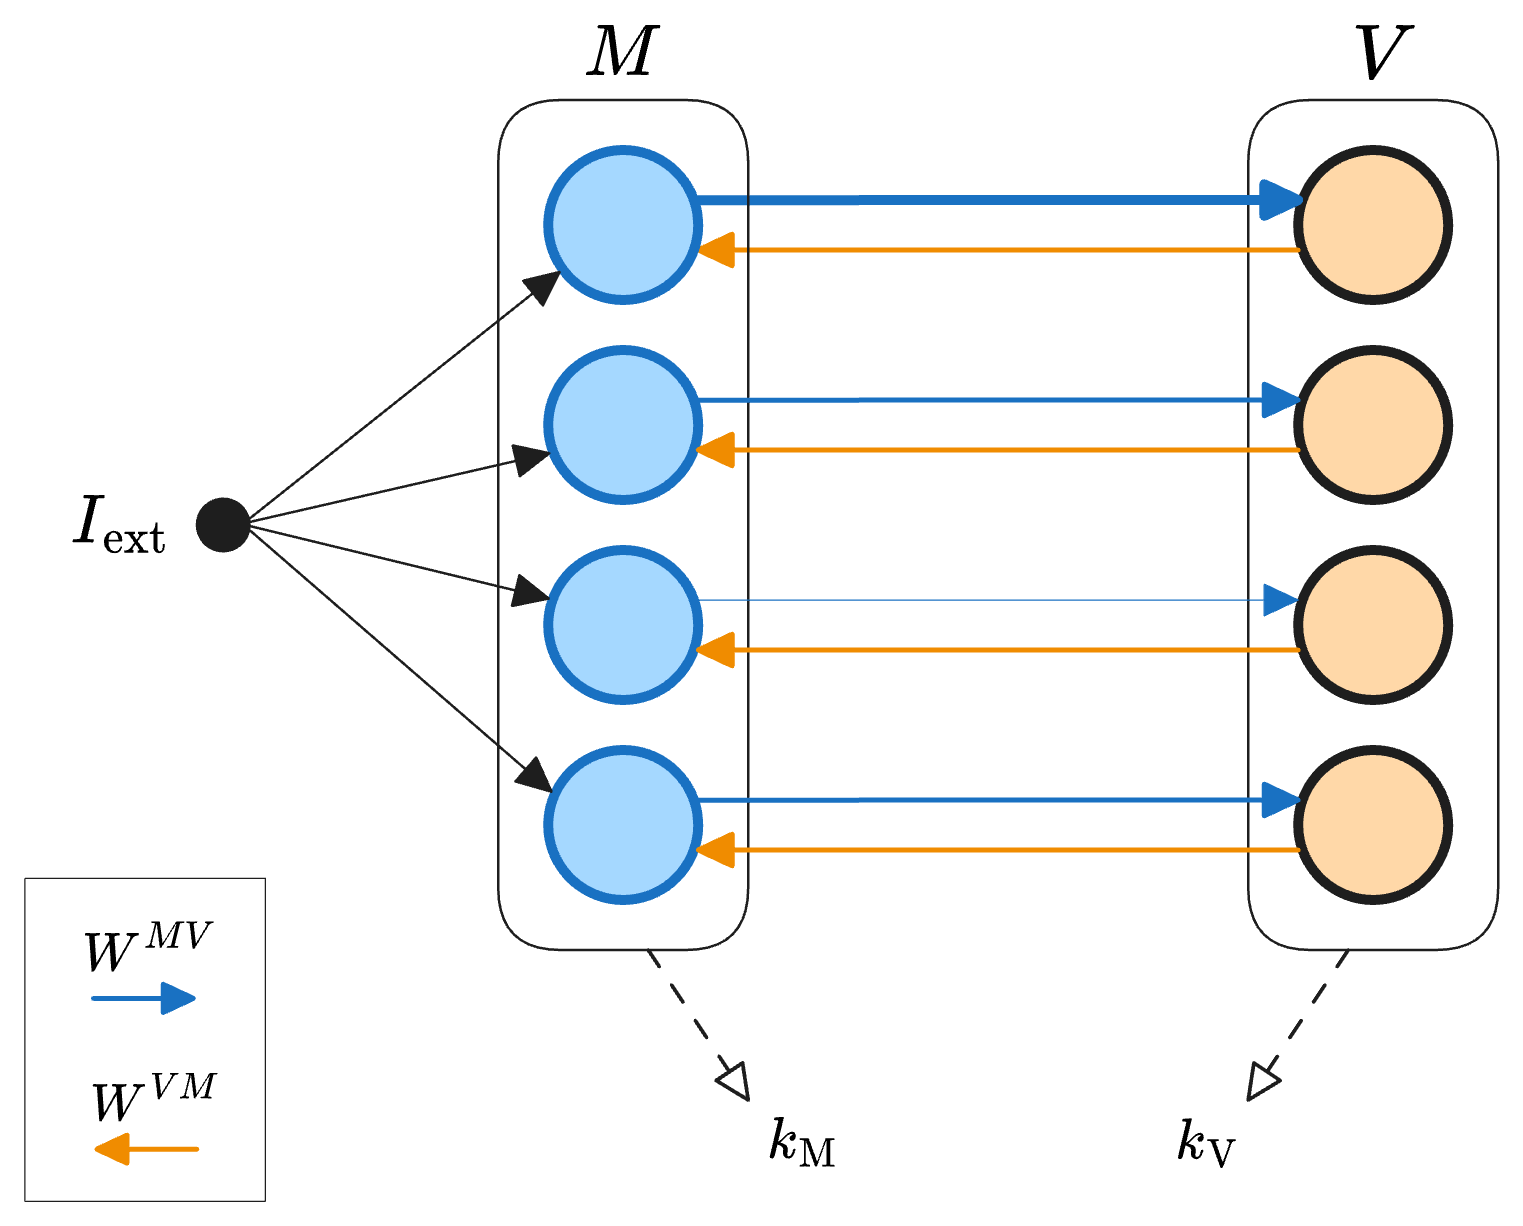
\includegraphics[width=0.6\textwidth]{figures/minb_architecture.png}
    \caption{\textsc{Model architecture} - \textit{The model is composed of a layer $M$ (blue), receiving a feedfoward input $I_{\text{ext}}$, a layer $V$ (orange), and connections $\textbf{W}^{MV}$ and $\textbf{W}^{VM}$. Additionally, two indexes $k_{M}, k_{V}$  can be extracted from the layers and
    corresponds to the selection made by the two populations as $k_{M}=\text{argmax}_{k} \{\textbf{u}\}$, $k_{V}=\text{argmax}_{k} \{\textbf{v}\}$.}}
    \label{fig:main_architecture}
\end{figure}

\noindent Importantly, the two layers are not fully connected and the matrices are diagonal. Further, the weight matrix $\textbf{W}^{VM}$ is simply the identity, while $\tilde{\textbf{W}}^{MV}$ is a function of the actual weights $\Phi_{v}(\textbf{W}^{MV})$ and it represents the contribution of the active options $\textbf{u}$ to the value representation $\textbf{v}$.
The function $\Phi_{v}$ is defined as the sum of a generalized sigmoid and a Gaussian, whose shape is characterized by a bell curve smoothly settling to a constant value. See more in the appendinx \ref{sec:appendix}.

\subsubsection{Option selection}
The decision-making process within a single round is structured in two distinct phases. Initially, the model receives a constant external input targeting all neurons in the memory population \textit{M} equally.
During this phase, $\textbf{I}_{\text{ext}}$ works as an equilibrium value while the reciprocal interactions with population \textit{V} push $\textbf{u}$ to different values, depending on the current policy encoded in $\tilde{\textbf{W}}^{MV}$. However, in the early rounds the weights $\textbf{W}^{MV}$ are zero, and thus
the contribution from \textit{V} is null. After a fixed amount of time $\sim 5 \text{s}$, the second phase begins. Here, the external input is removed and the model is left to evolve autonomously, and since there are no recurrent connections in neither population the dynamics are entirely driven by their coupling. A selection $k$ is sampled after another fixed amount of time $\sim 5 \text{s}$, and it is defined according to the following rule:

\begin{equation*}
    k =
    \left\{
        \begin{array}{ll}
            \text{argmax}_{k}\{\textbf{v}\} & \text{\textit{if}}\; \text{argmax}_{k} \{\textbf{v}\} = \text{argmax}_{k} \{\textbf{u}\} \\
            \text{random}(K) & \text{\textit{otherwise}}
        \end{array}
    \right.
\end{equation*}

\noindent The selection rule is simple: if the value representation $\textbf{v}$ is in agreement with the memory trace $\textbf{u}$, then the option with the highest value is selected. Otherwise, a random option is chosen. This rule is a way to express the exploration-exploitation trade-off, and it
is dependent on the current policy $\tilde{\textbf{W}}^{MV}$. \\ Below \ref{alg:decision1}, is reported the pseudo-code for algorithm behind the selection process.

% --- ALGORITHM
\begin{algorithm}[ht]
\caption{Two-phases option selection process}
\label{alg:decision}
\SetAlgoLined
\KwIn{External input $\textbf{I}_{\text{ext}}$, population $\textbf{u}$, population $\textbf{v}$, weights $\tilde{\textbf{W}}^{MV}$}
\KwOut{Selected action $k$}

\SetKwComment{Comment}{// }{ }

\textbf{Phase 1:} \textit{external input} \Comment*[r]{Duration: $\sim$5s}
Define constant $\textbf{I}_{\text{ext}}$\;
Update populations $\textbf{u}, \textbf{v}$ according to \ref{eq:main}\;

\textbf{Phase 2:} \textit{autonomous evolution} \Comment*[r]{Duration: $\sim$5s}
Remove external input $\textbf{I}_{\text{ext}}$\;
Let system evolve through population coupling according to \ref{eq:main}\;

\textbf{Selection process:}\;
$k_{u} \gets \text{argmax}_{k}\{\textbf{u}\}$\;
$k_{v} \gets \text{argmax}_{k}\{\textbf{v}\}$\;
\eIf{$k_{u} = k_{v}$}{
    $k \gets k_{v}$ \Comment*[r]{Exploitation}}{
    $k \gets \text{random}(K)$ \Comment*[r]{Exploration}
}
\Return $k$
\end{algorithm}\label{alg:decision1}

\noindent In figure \ref{fig:sel1} it is shown the history of selections over three trials. The initial rounds features higher variability. In particular, it can noted how the policy adopted by the model encounters period of exploration and successive settling over an explotative strategy, which can be reverted in case of a change in the environment's reward distribution.

% selections over time
\begin{figure}[ht]
    \centering
    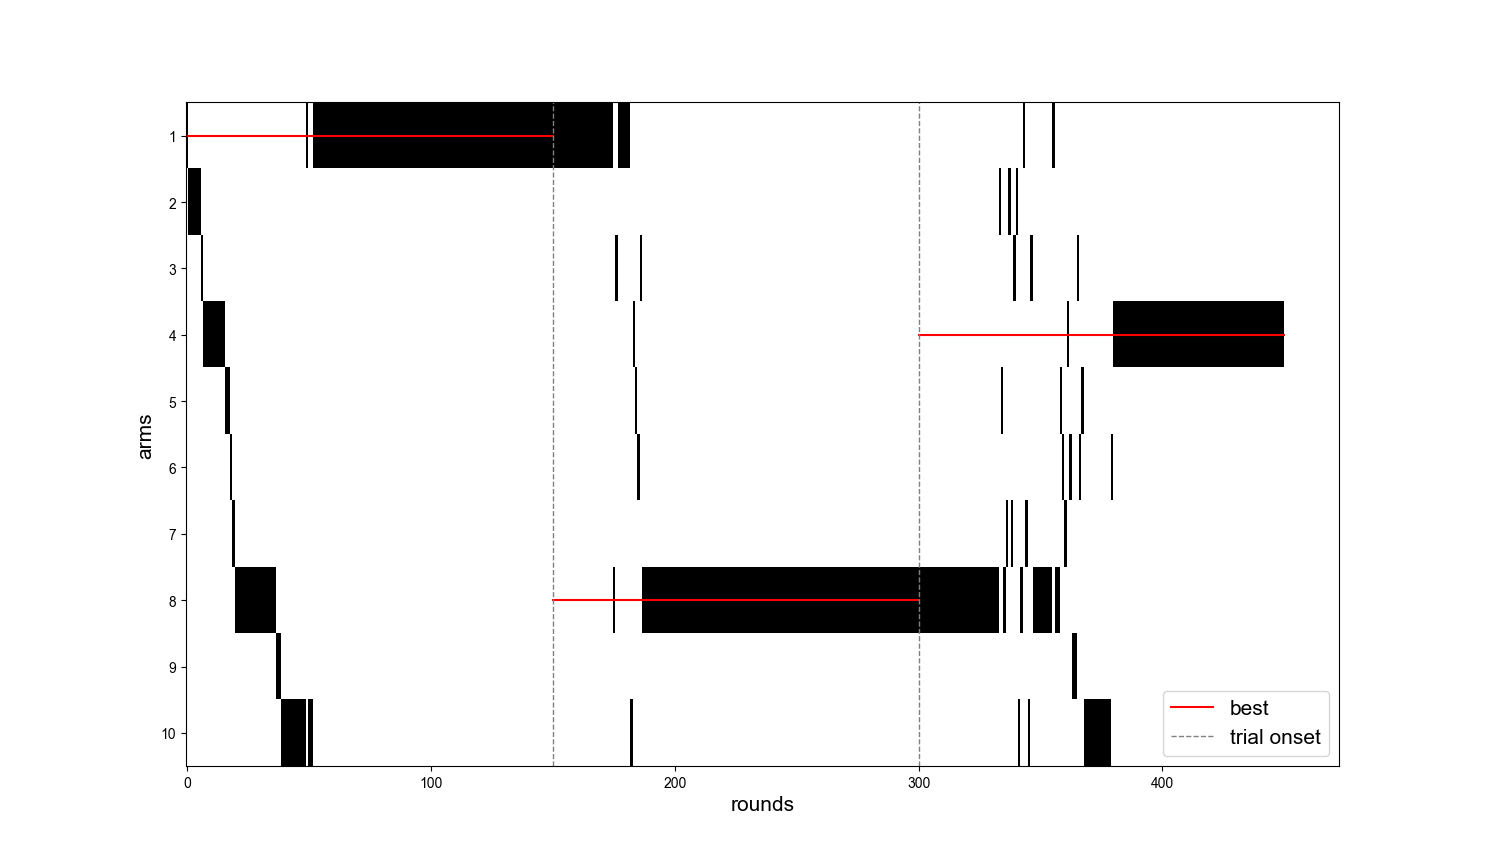
\includegraphics[width=0.9\textwidth]{figures/selections_1.png}
    \caption{\textsc{Selection evolution over rounds} - \textit{the x-axis represents the available arms, while the y-axis the number of rounds, with the dotted vertical lines indicating the start of a new trial with 150 rounds each.
The model selections are the black vertical lines for an arm and a round. The red horizontal lines signal the arm with the highest reward probability, thus representing the best (and greediest) selection.}}
    \label{fig:sel1}
\end{figure}


\subsection{Learning}
Given a selected option $k$, the environment (set of bandits) samples and returns a reward $R\in [0, 1]$ with probability $p_{k}$.
Then, the connections $\textbf{W}^{MV}$ for the neuron corresponding to the option $k$ are updated according to the following plasticity rule:

\begin{equation}
    \Delta \textbf{W}^{MV}_{k} = \tilde{\eta}_{k} \left(R\cdot W^{+}- \textbf{W}^{MV}_{k}\right)
\end{equation}

\noindent
Where $W^{+}$ is a constant value that sets the upper bound for the synaptic weights, and it is set to $W^{+} = 5$, while $\tilde{\eta}_{k}$ is the learning rate for the option $k$ determined by a function of the current weights $\textbf{W}^{MV}_{k}$ and its shape is the same as $\Phi_{v}$, but with
different parameters.


\subsection{Bio-inspired features}

The model is inspired by the functioning of the prefrontal cortex (PFC) and its importance in decision-making processes. In particular, despite their marked simplicity, the two population $M, V$ of the model can be related to the orbito-frontal cortex (OFC) and anterior cingulate cortex (ACC), respectively.
More specifically, the OFC is known to be involved in the representation of the state different options and update their value with respect to rewarding outcomes and their history \cite{lukChoiceCodingFrontal2013, kennerleyDecisionMakingReward2011a}. The ACC has been associated to action values, and the dynamic interplay with OFC is observed to elicit
transient pre-stimulus activation, which biases the decision towards the most valuable option \cite{funahashiPrefrontalContributionDecisionMaking2017, marcosDeterminingMonkeyFree2016, balewskiValueDynamicsAffect2023}. In the model, the first layer represents the available options, while the learned
connections with the second layer encode their values based on the recent reward history. Another similarity with this particular pre-frontal circuit is the realization of a choice as a sample of the network state after a period of autonomous neural activity, where the depth of the closest
neural attractor depends on the strength and reliability of the highest option value \cite{backmanEffectsWorkingMemoryTraining2011, enelStableDynamicRepresentations2020}.

